% Template used by paper.py; paper.tex is generated from it.
\documentclass[conference]{IEEEtran}
\IEEEoverridecommandlockouts
\usepackage[utf8]{inputenc}
\usepackage[T1]{fontenc}
\usepackage{cite}
\usepackage{amsmath,amssymb}
\usepackage{graphicx}
\usepackage{booktabs}
\usepackage{url}
\usepackage[hidelinks]{hyperref}
\usepackage{microtype}

\begin{document}

\title{Day-Ahead Load Forecast Accuracy of U.S. Balancing Authorities, 2015--2026:\\ A Scorecard from Public EIA-930 Data\\
\large Cardinal Grid Notes, No.\ 1 (draft of <<generated>>)}

\author{\IEEEauthorblockN{Ricardo W. C. Guerra Filho}
\IEEEauthorblockA{Cardinal Grid (independent open initiative)\\
ORCID 0000-0001-6699-9951 \quad contact@cardinalgrid.com}}

\maketitle

\begin{abstract}
Balancing authorities (BAs) in the contiguous United States report to the U.S. Energy Information Administration, through Form EIA-930, both the hourly demand that occurred and the day-ahead demand forecast they produced the previous day. This note scores those forecasts for the full public record, from <<first_prose>> to <<last_prose>>. For each BA-day with at least 20 valid hours, mean absolute percentage error (MAPE), bias, root-mean-square error and the error at the hour of the actual daily peak are computed after explicit data-quality rules. Of <<n_total>> BAs in the files, <<n_scored>> report both series and <<n_eligible>> meet the eligibility criteria for ranking. The demand-weighted day-ahead MAPE across eligible BAs is <<dw_mape>>, with a median BA value of <<med_mape>>. At the hour of the daily peak, the forecast was below actual demand on <<under_share>> of eligible BA-days, and the share has increased since 2019; one eligible BA-day in a hundred under-forecasts the peak by more than <<p99>>. The highest error values in the ranking are dominated by reporting problems rather than forecasting problems, which motivates the data-quality layer of the underlying tool. Code, results and the event calendar are archived with a DOI.
\end{abstract}

\begin{IEEEkeywords}
load forecasting, balancing authority, EIA-930, forecast evaluation, data quality, bulk power system reliability
\end{IEEEkeywords}

\section{Introduction}
The day-ahead load forecast is the quantity against which a balancing authority commits generation and procures operating reserves. When the forecast is below the load that occurs, reserves are short; the joint FERC--NERC inquiry into Winter Storm Elliott documented day-ahead under-forecasts of up to 11.6\% at one BA, with a mean absolute error approaching 10\% across BAs, contributing to emergency operations and firm load shed \cite{ferc2023elliott}. The Commission's review of the January 2024 Arctic storms found operators discarding genuinely high load readings as bad data \cite{ferc2024arctic}. NERC's 2025 Long-Term Reliability Assessment projects summer peak demand growth of 224~GW over ten years and states that traditional load forecasting methods may not be sufficient to capture the speed and uncertainty of large-load additions \cite{nerc2026ltra}; the U.S. Department of Energy estimates that, absent corrective action, outage risk could increase roughly 100-fold by 2030 \cite{doe2025reliability}.

These findings concern specific events. A systematic, public measurement of day-ahead forecast accuracy across all BAs has been possible since July 2015, when EIA began collecting hourly demand and the day-ahead demand forecast from every BA in the contiguous United States \cite{eia930monitor}. This note presents that measurement for the full record to date, using an open-source tool \cite{guerra2026scorecard}, and reports three results: the distribution of forecast error across BAs, the accuracy of the largest operators, and a systematic tendency to under-forecast the daily peak hour. The purpose is descriptive. No BA has been contacted, and the note does not attempt to explain any individual BA's performance.

\section{Data}
\subsection{Source and definitions}
Form EIA-930 requires each NERC-registered BA to report, in a daily file due by 7:00~a.m.\ Eastern, ``yesterday's hourly day-ahead demand forecast for today'' and the hourly demand that occurred, as ``hourly integrated values in megawatts by hour ending time'' with UTC time stamps \cite{eia930instructions}. The instructions define the forecast field only as ``the day-ahead demand forecast'' and state that a BA which does not produce a forecast directly comparable to reported demand should report ``the day-ahead demand forecast generated in the normal course of business''. EIA therefore prescribes neither the forecasting method, nor its inputs, nor the time of day at which the forecast is produced. The forecast series is each BA's operational day-ahead forecast as it existed the day before, at that BA's own cut-off time.

\subsection{Coverage}
The analysis uses EIA's six-month balance files from <<first_prose>> to <<last_prose>> \cite{eia930monitor}, which contain <<n_total>> BA codes. Generation-only BAs report no demand and are excluded automatically. <<n_scored>> BAs report both demand and forecast for enough hours to be scored. EIA's own imputation flag for demand is retained; imputed values account for <<imputed>> of scored hours.

\section{Methods}
\subsection{Metrics}
Let $D_h$ and $F_h$ be demand and forecast in hour $h$ of a BA-day, and $e_h = F_h - D_h$ (positive values are over-forecasts). For each BA-day with a set $H$ of valid hours,
\begin{align}
\mathrm{MAPE} &= \frac{1}{|H|}\sum_{h\in H} \frac{|e_h|}{D_h}, &
\mathrm{bias} &= \frac{1}{|H|}\sum_{h\in H} \frac{e_h}{D_h}, \\
\mathrm{RMSE} &= \sqrt{\frac{1}{|H|}\sum_{h\in H} e_h^2}, &
\epsilon_{\mathrm{peak}} &= \frac{e_{h^\ast}}{D_{h^\ast}},\; h^\ast = \arg\max_{h\in H} D_h .
\end{align}
The peak-hour error $\epsilon_{\mathrm{peak}}$ is the error at the hour of the actual daily peak, which is the quantity relevant to reserve adequacy. BA-day values are aggregated over months, years and the whole period as hour-weighted means; the demand-weighted MAPE across BAs weights each BA-day by its mean demand and its number of valid hours.

\subsection{Data-quality rules}
Three rules are applied before any error is computed. (i)~Hours with $D_h \le 0$ or $F_h \le 0$ are excluded. (ii)~Hours with $F_h/D_h$ outside $[1/2, 2]$ are flagged as implausible and excluded: the band retains every documented extreme-weather miss, including the 11.6\% Elliott case, and removes unit errors, partial reports and stale values. (iii)~A BA-day is scored only if it has at least 20 valid hours. In addition, a BA whose median daily bias over the whole period exceeds $\pm 25\%$ is treated as a series mismatch, in which forecast and demand do not describe the same quantity, and is listed separately rather than ranked. Over the period, <<implausible>> hours were flagged under rule (ii), and <<mismatch>> were excluded as series mismatches.

\subsection{Eligibility and events}
BAs enter the ranking if they have at least 180 scored days, a mean demand of at least 500~MW, and no series mismatch; <<n_eligible>> BAs qualify. Named events are fixed date windows taken from the public inquiries: Winter Storm Uri (13--20 February 2021), the Pacific Northwest heat dome (26--30 June 2021), Winter Storm Elliott (23--26 December 2022), the July--August 2023 heat wave, the January 2024 Arctic storms (13--17 January 2024) and the January 2025 cold wave (19--24 January 2025), each restricted to the EIA regions the inquiries identify.

\section{Results}
\subsection{Distribution of forecast error across BAs}
Table~\ref{tab:summary} summarizes the period. Fig.~\ref{fig:ranking} shows the whole-period MAPE of every eligible BA. The demand-weighted MAPE is <<dw_mape>> and the median BA is at <<med_mape>>. The five lowest values are <<top>>; the five highest are <<bottom>>.

\begin{table}[t]
\caption{Summary of the scored record, <<first_month>> to <<last_month>>.}
\label{tab:summary}
\centering
\begin{tabular}{lr}
\toprule
Quantity & Value \\
\midrule
BAs in the EIA-930 files & <<n_total>> \\
BAs reporting demand and forecast & <<n_scored>> \\
BAs eligible for ranking & <<n_eligible>> \\
BA-days scored & <<ba_days>> \\
Hours scored & <<hours>> \\
Hours flagged implausible & <<implausible>> \\
Demand-weighted MAPE, eligible BAs & <<dw_mape>> \\
Median BA MAPE, eligible BAs & <<med_mape>> \\
BA-days with forecast below peak-hour demand & <<under_share>> \\
1st percentile of peak-hour error & $-$<<p99>> \\
\bottomrule
\end{tabular}
\end{table}

\begin{figure*}[t]
\centering
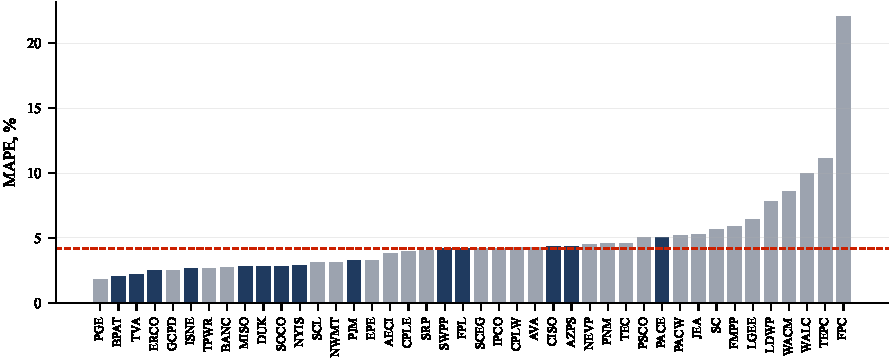
\includegraphics[width=\textwidth]{figures/fig1_ranking.pdf}
\caption{Whole-period hour-weighted day-ahead MAPE of the <<n_eligible>> eligible balancing authorities, <<first_month>> to <<last_month>>, sorted by value; the dashed line is the median. Filled bars are the largest ISOs/RTOs and utilities listed in Table~\ref{tab:major}. Source: EIA-930 six-month files \cite{eia930monitor}; scoring by \cite{guerra2026scorecard}.}
\label{fig:ranking}
\end{figure*}

\subsection{The largest operators}
Table~\ref{tab:major} reports the largest ISOs/RTOs and utilities. Fig.~\ref{fig:yearly} shows their yearly MAPE. Two features of Fig.~\ref{fig:yearly} are noted without interpretation: the increase in the yearly MAPE of CISO and SWPP since 2023, and the 2015 value of AZPS; each may reflect forecasting, a change in what the BA reports, or both. <<partial_year_note>>

\begin{table}[t]
\caption{Largest balancing authorities: whole-period day-ahead forecast error. Rank is among the <<n_eligible>> eligible BAs. The last column is the 1st percentile of the peak-hour error, i.e. the under-forecast exceeded on one BA-day in a hundred.}
\label{tab:major}
\centering
\small
\begin{tabular}{rllrrrr}
\toprule
Rank & BA & Region & MAPE & Bias & $|\epsilon_{\mathrm{peak}}|$ mean & $P_{1}(\epsilon_{\mathrm{peak}})$ \\
\midrule
<<major_rows>>
\bottomrule
\end{tabular}
\end{table}

\begin{figure}[t]
\centering
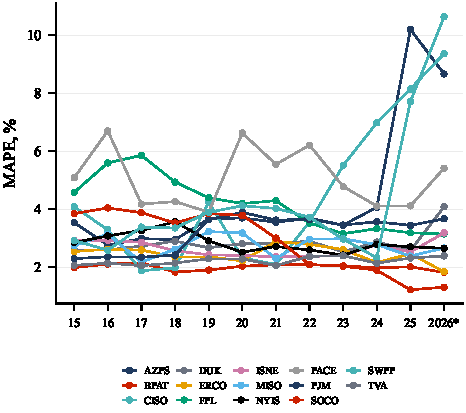
\includegraphics[width=\columnwidth]{figures/fig2_yearly_major.pdf}
\caption{Yearly hour-weighted MAPE of the largest balancing authorities. <<partial_year_note>>}
\label{fig:yearly}
\end{figure}

\subsection{Peak-hour bias}
Fig.~\ref{fig:peak} shows, for each year, the share of eligible BA-days on which the forecast at the hour of the actual daily peak was below the demand that occurred. Over the whole period the share is <<under_share>>; an unbiased forecast would give a value near 50\%. The share has increased since 2019 and exceeded 60\% in every year from 2023. The first percentile of the peak-hour error across all eligible BA-days is $-$<<p99>>.

\begin{figure}[t]
\centering
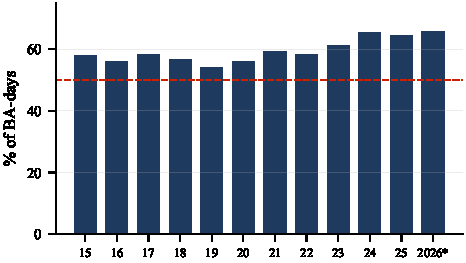
\includegraphics[width=\columnwidth]{figures/fig3_peak_under_forecast_share.pdf}
\caption{Share of eligible BA-days on which the day-ahead forecast was below actual demand at the hour of the daily peak, by year. The dashed line marks 50\%. <<partial_year_note>>}
\label{fig:peak}
\end{figure}

\subsection{Named events}
Table~\ref{tab:events} lists, for each event window, the eligible BA with the largest peak-hour under-forecast, and Fig.~\ref{fig:events} shows the distribution across eligible BAs. The largest single eligible BA-day miss in the record is <<worst_ba>> on <<worst_date>>, a forecast <<worst_pct>> below a <<worst_mw>>~MW peak; single-day extremes of this size may still be reporting problems, and the percentile statistics above are the robust figures.

\begin{table}[t]
\caption{Largest peak-hour under-forecast by an eligible BA during each named event window.}
\label{tab:events}
\centering
\small
\begin{tabular}{llr}
\toprule
Event & BA (region) & Under-forecast at peak \\
\midrule
<<event_rows>>
\bottomrule
\end{tabular}
\end{table}

\begin{figure}[t]
\centering
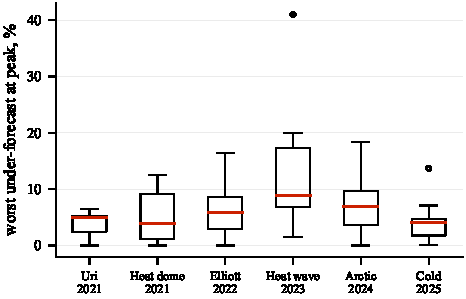
\includegraphics[width=\columnwidth]{figures/fig4_events.pdf}
\caption{Distribution across eligible BAs of the worst peak-hour under-forecast within each named event window (0 means the BA never under-forecast the peak during the window).}
\label{fig:events}
\end{figure}

\section{Discussion}
\subsection{Interpretation}
Three points follow from the results. First, typical day-ahead accuracy is a few percent, and the largest operators are at or below the median; the long tail of the ranking is, on inspection, a tail of reporting quality rather than of forecasting skill, which is why the scoring tool carries an explicit data-quality layer and why the highest values should be read as ``data or forecast problem'', not ``forecast problem''. Second, the peak-hour bias is systematic and has grown: on roughly six BA-days in ten the forecast used for reserve procurement was below the load that occurred at the peak, and the share has risen through the period of rapid large-load growth. The mechanism is not identified here; candidate explanations include structural load growth outpacing model updates and asymmetric loss functions in operational practice. Third, event windows show that misses of 10--20\% at the peak hour are not confined to the Elliott case documented by FERC and NERC.

\subsection{Limitations}
Forecasts are as submitted to EIA and may differ from what operators used internally; EIA's revision rules apply to measured data, not to the forecast. The forecast horizon is not the same for every BA: a forecast closed at 9~a.m.\ the day before covers 15 to 39 hours ahead, one closed at 5~p.m.\ covers 7 to 31, and EIA does not record the cut-off time, so part of the difference between BAs is horizon rather than skill; comparisons of a given BA over time are not affected. Several small BAs' series contain errors that the plausibility band does not catch. Event windows are fixed dates rather than weather-defined extreme days. No BA has been contacted for comment.

\section{Conclusion}
The public EIA-930 record allows the day-ahead load forecasts of every U.S. balancing authority to be scored continuously without any operator's cooperation. Over <<first_month>> to <<last_month>>, eligible BAs show a demand-weighted day-ahead MAPE of <<dw_mape>>, a systematic and growing tendency to under-forecast the daily peak hour, and a tail of apparent errors that are reporting problems. The scoring tool, its results and the event calendar are open and updated daily, and subsequent notes will address data quality in the EIA-930 series and the attribution of errors to weather.

\section*{Data and Code Availability}
Data: EIA-930 six-month balance files \cite{eia930monitor}. Code and results: \cite{guerra2026scorecard} (Apache-2.0), archived at \url{https://doi.org/10.5281/zenodo.22697386}. This note and its figures are reproduced by \texttt{analysis.py} and \texttt{paper.py} in \url{https://github.com/cardinalgrid/notes}.

\bibliographystyle{IEEEtran}
\bibliography{references}

\end{document}
